% ============================================================================
%  Cell-state reachability: a convex-cone oracle for feasibility verdicts
%  Preprint manuscript — compiled with tectonic (pdflatex-compatible)
% ============================================================================
\documentclass[11pt]{article}

% ---- Geometry: preprint single-column ----
\usepackage[letterpaper,margin=1in]{geometry}
\usepackage[T1]{fontenc}
\usepackage[utf8]{inputenc}
\usepackage{lmodern}
\usepackage{microtype}

% ---- Math ----
\usepackage{amsmath,amssymb,amsthm}
\usepackage{bm}

% ---- Figures & tables ----
\usepackage{graphicx}
\graphicspath{{figures/}}
\usepackage{booktabs}
\usepackage{array}
\usepackage{caption}
\usepackage{subcaption}
\captionsetup{font=small,labelfont=bf}
\captionsetup[sub]{font=footnotesize}

% ---- Float placement: let large figures settle near their text ----
\usepackage{placeins}
\renewcommand{\topfraction}{0.9}
\renewcommand{\bottomfraction}{0.85}
\renewcommand{\textfraction}{0.08}
\renewcommand{\floatpagefraction}{0.7}
\setcounter{topnumber}{2}
\setcounter{totalnumber}{3}

% ---- Colours & links ----
\usepackage{xcolor}
\definecolor{linkblue}{HTML}{2166AC}
\usepackage[colorlinks=true,allcolors=linkblue,breaklinks=true]{hyperref}
\usepackage{url}

% ---- Bibliography: natbib numeric ----
\usepackage[numbers,sort&compress,comma]{natbib}
\bibliographystyle{unsrtnat}

% ---- Headers ----
\usepackage{fancyhdr}
\pagestyle{fancy}
\fancyhf{}
\rhead{\small Cell-state reachability oracle}
\lhead{\small Preprint}
\cfoot{\thepage}
\renewcommand{\headrulewidth}{0.2pt}

% ---- Theorem-like environments (used lightly in Methods) ----
\newtheorem{definition}{Definition}
\newtheorem{proposition}{Proposition}

% ---- Convenience macros ----
\newcommand{\reach}{\textsc{Reach}}
\newcommand{\cone}{\mathcal{C}}
\newcommand{\Emat}{\mathbf{E}}
\newcommand{\dvec}{\mathbf{d}}
\newcommand{\wvec}{\mathbf{w}}
\newcommand{\Rnn}{\mathbb{R}_{\geq 0}}
\newcommand{\Th}[1]{T\textsubscript{H}#1}

% ---- Title ----
\usepackage{authblk}
\title{\bfseries A convex-cone reachability oracle for cell-state engineering:\\
falsifiable feasibility verdicts and constructive certificates\\
from measured genome-scale perturbation screens}

\author[1]{Cell-State Reachability Project}
\affil[1]{\small Built with Claude --- Life Sciences (Research track)}
\date{\today}

% ============================================================================
\begin{document}
\maketitle

\begin{abstract}
\noindent
Deciding whether a desired change in cell state can be produced by a given class of
perturbation---and, if not, saying so before the experiment is run---is the central
question of cell-state engineering and of pharmaceutical target selection. Existing
computational methods either predict the response to a specified perturbation or rank
candidate regulators; none returns a \emph{feasibility verdict} grounded in measured
effects, and none can certify that a goal is unreachable. We introduce a convex-cone
reachability oracle that treats a genome-scale CRISPRi Perturb-seq screen as a dictionary
of measured effect vectors and asks whether a target cell-state shift lies in their
non-negative combination. Because loss-of-function knockdowns combine additively and
non-negatively, reachability is membership in a convex cone, decided by non-negative least
squares; a reachable target yields a minimal ranked knockdown recipe, and an unreachable
target yields a Farkas/KKT separating-hyperplane certificate that names the genes which
would instead have to be \emph{activated}---a falsifiable gain-of-function hypothesis rather
than a null result. Applied to a screen in primary human CD4\textsuperscript{+} T cells,
the oracle finds the T\textsubscript{H}2$\rightarrow$T\textsubscript{H}1 polarization shift
partly reachable by knockdown (held-out cosine $0.448$ against a shuffled-target null of
$-0.005$, $z\approx24$), with a signed decomposition attributing 39\% of the shift to
loss-of-function, 25\% to required activation, and 35\% to an irreducible remainder;
canonical regulators appear as expected positive controls (GATA3 reached, TBX21
correctly anti-aligned). Across a 12-cell atlas of four transitions under three activation
states, knockdown is never the majority modality (mean loss-of-function fraction $0.34$).
The same operator transfers unchanged to a K562 CRISPRa combinatorial screen (held-out
CEBPA cosine $0.878$), whose measured double perturbations show that the additivity
assumption is a bounded approximation (median cosine $0.71$ to the sum of singles) rather
than an identity. Against a 92-method survey (2011--2026), measured-effect grounding and a
feasibility verdict with a certificate are held by disjoint sets of prior methods; their
intersection is empty. The verdict is stable under stress: it strengthens rather than weakens
when the metric is reweighted by target magnitude to guard against signal dilution, the
non-negativity constraint costs little in fit yet supplies the certificate, and a
cross-cell-type probe shows that the \emph{direction} of a shift transfers across cell types
while the specific minimal \emph{recipe} does not. The oracle is a hypothesis-prioritization and experiment-triage
instrument---it decides where a screen should spend its arms and where it should stop---not
a target-validation engine, and every nomination is a falsifiable wet-lab hypothesis.
\end{abstract}


\section{Introduction}
\label{sec:intro}

Much of experimental biology is a search for interventions that move a cell from one state
to another: differentiating a stem cell, repolarizing a T cell, reverting a diseased
phenotype, or---in drug discovery---knocking down a target to reverse a pathogenic program.
Before committing reagents to such a program, the decisive question is not \emph{what will
this perturbation do} but \emph{can the desired change be achieved at all with the
perturbations available, and if not, what is missing}. That question is rarely asked
computationally, and its economic weight is large: only about one in ten clinical
programs succeeds and many late-stage failures involve insufficient efficacy. That clinical
context motivates better early evidence, but a transcriptomic screen cannot by itself explain
or prevent clinical attrition. Human genetic support and directly measured target effects do,
however, both argue for grounding target choice in real perturbation data rather than inferred
models \citep{Minikel2024,Nelson2015,Harrison2016,%
BegleyEllis2012,Prinz2011}.

The computational tools available to answer it fall into two camps that, as we document in
Section~\ref{sec:related}, do not overlap. Perturbation-response models---from
gene-regulatory-network simulators to single-cell foundation models---are increasingly
trained on real screens but are forward predictors: given a perturbation they return a
predicted response, and a predictor structurally always returns \emph{some} answer, so it
cannot certify that a goal is out of reach. Network-control and Boolean-attractor methods
do reason about reachability and can carry controllability guarantees, but those guarantees
are properties of a hand-built or inferred model, only as trustworthy as the network
assumed. Neither camp answers the feasibility question from measured effects. This gap
matters all the more because a wave of 2025--2026 benchmarks finds that current
perturbation predictors, foundation models included, frequently fail to beat mean or linear
baselines on genuinely unseen perturbations \citep{AhlmannEltze2025,Wong2025,Kernfeld2025,%
Atti2025}: the field's own evidence argues for an output weaker and more defensible than
predicting an unseen response.

\paragraph{The convex-cone move.}
We take the opposite starting point from model building: we do not infer a network at all.
A genome-scale CRISPRi Perturb-seq screen \citep{Zhu2025} directly measures, for each
perturbation--condition profile, the effect vector it produces in expression
space. We treat these measured vectors as a fixed dictionary and ask a geometric question:
does the desired cell-state shift lie in the set of shifts the dictionary can produce?
Two modelling choices make this a convex-geometry problem. A measured knockdown effect may be
applied with non-negative weight but not reversed into an unmeasured ``negative knockdown'';
and several knockdowns are approximated, to first order, by the sum of their single effects.
Individual effect vectors may raise some transcripts and lower others. The set of directions
allowed by this model is therefore the \emph{non-negative conic hull} of
the measured effect vectors, and asking whether a target is reachable is asking whether it
lies inside that model-relative cone---a question non-negative least squares (NNLS) answers exactly
\citep{LawsonHanson1974}. This reframing turns an open-ended design search into a decision
with a checkable solution on both sides. When the target is inside the cone, the NNLS weights
rank a feasible mixture and a greedy spectrum supplies compact candidate panels; neither is a
global minimum-cardinality proof. When it is outside, convex duality supplies a separating
hyperplane---a Farkas/KKT certificate \citep{Farkas1902,KuhnTucker1951}---whose full vector
certifies the mismatch. Positive coordinates rank readouts under-delivered at the closest cone
point. They motivate a CRISPRa or de-repression arm, but do not prove that activating any
individual readout will cause the desired state.

\paragraph{Scope.}
The oracle is a decision instrument, not an oracle of biological truth: it certifies
feasibility \emph{relative to the measured dictionary} under an explicit additivity model, and
its verdicts are hypotheses for the bench, not validated targets. The regulators it surfaces in
T cells and in the CEBPA program are already reported by the source screens
\citep{Zhu2025,Norman2019} and enter here only as positive controls; the novelty we claim is
the measured-effect, certificate-carrying reachability \emph{decision} itself, not the biology
it recovers.

\paragraph{Contributions.}
This paper makes four contributions.
\begin{enumerate}
\item \textbf{A feasibility oracle for cell-state engineering.} We formalize reachability of
a target cell-state direction as membership in the convex cone of measured perturbation effect
vectors, and solve it with NNLS so that a verdict, a ranked mixture, a greedy sparse panel,
and---on infeasibility---a Farkas/KKT dual certificate follow from one convex program
(Section~\ref{sec:methods}).
\item \textbf{A validated headline result.} On primary human
CD4\textsuperscript{+} T cells the oracle finds T\textsubscript{H}2$\rightarrow$%
T\textsubscript{H}1 partly reachable by knockdown---far above a shuffled-target null but well
below full reachability---with a signed loss-/gain-of-function decomposition and canonical
regulators recovered as positive controls (Section~\ref{sec:results-headline}).
\item \textbf{Generality across transitions and datasets.} A 12-cell atlas shows knockdown
is never the majority modality across four transitions and three activation states, and the
identical operator runs without retuning on a K562 CRISPRa combinatorial screen, where
we also quantify the additivity approximation directly on measured doubles
(Sections~\ref{sec:results-atlas}--\ref{sec:results-transfer}).
\item \textbf{An exact positioning against the literature.} Over 92 methods spanning
2011--2026, we show that measured-effect grounding and feasibility-with-certificate are held
by disjoint method sets whose intersection is empty, and translate the resulting verdicts
into a GO/REDIRECT/STOP triage over 102 real target nominations
(Sections~\ref{sec:results-landscape}--\ref{sec:results-impact}).
\end{enumerate}


\input{sections/20_methods}

\section{Results}
\label{sec:results}

Figure~\ref{fig:framework} summarizes the framework: a genome-scale screen yields measured
effect vectors (\ref{fig:framework}A); reachability is membership in their convex cone, with
the residual naming what knockdown cannot supply (\ref{fig:framework}B); a reachable target
returns a verdict, a signed decomposition, and an activation certificate
(\ref{fig:framework}C); and the same operator transfers to an independent screen
(\ref{fig:framework}D).

\begin{figure}[htbp]
\centering
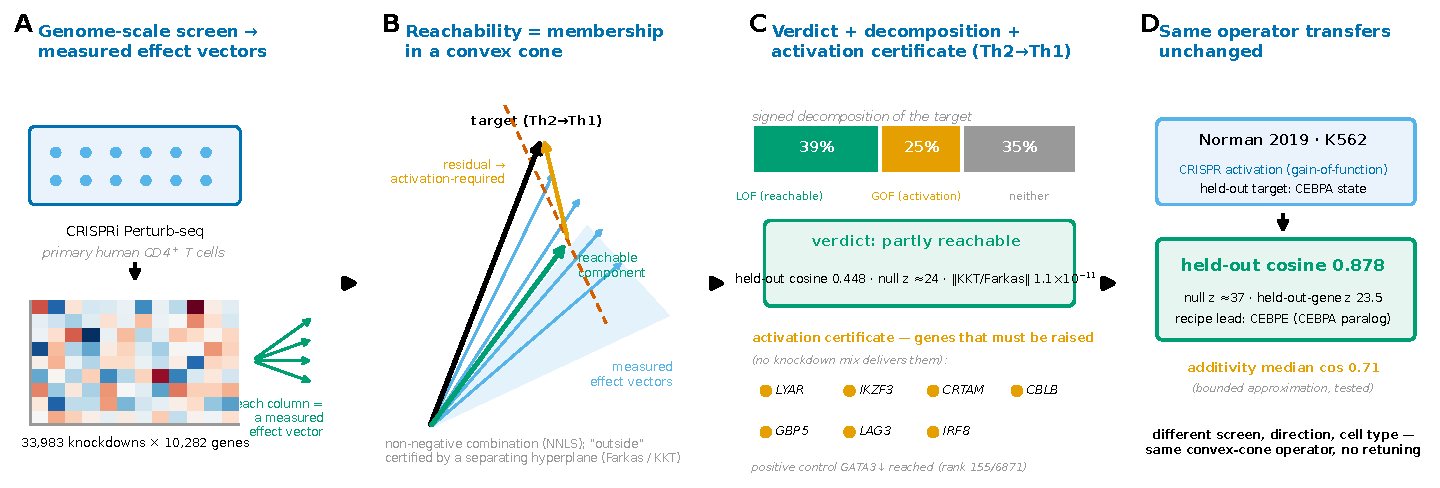
\includegraphics[width=\textwidth]{fig1}
\caption{\textbf{The convex-cone reachability oracle.}
\textbf{(A)}~A genome-scale CRISPRi Perturb-seq screen in primary human
CD4\textsuperscript{+} T cells yields, for each of $33{,}983$ knockdowns, a measured effect
vector over $10{,}282$ genes. \textbf{(B)}~Reachability is membership in the non-negative
conic hull of these vectors; the reachable component is the NNLS projection of the target,
and the residual is the activation-required direction, with ``outside'' certified by a
separating hyperplane (Farkas/KKT). \textbf{(C)}~For
T\textsubscript{H}2$\rightarrow$T\textsubscript{H}1 the oracle returns a
\emph{partly reachable} verdict (held-out cosine $0.448$, $\lVert$KKT/Farkas$\rVert\approx
1.1\times10^{-11}$), a signed decomposition ($39\%$ LOF / $25\%$ GOF / $35\%$ neither), and an
activation certificate naming genes that must be raised. \textbf{(D)}~The identical operator,
with no retuning, transfers to the Norman K562 CRISPRa screen (held-out CEBPA cosine
$0.878$).}
\label{fig:framework}
\end{figure}

\subsection{The T\texorpdfstring{\textsubscript{H}}{H}2\texorpdfstring{$\rightarrow$}{->}T\texorpdfstring{\textsubscript{H}}{H}1 shift is partly reachable by knockdown}
\label{sec:results-headline}
Our headline target is the T\textsubscript{H}2$\rightarrow$T\textsubscript{H}1 polarization
shift in resting cells, a canonical and therapeutically relevant repolarization. The greedy
reachability spectrum (Fig.~\ref{fig:headline}a) rises rapidly and plateaus: the reachable
cosine reaches a knee at $k=7$ knockdowns (cosine $0.40$) and saturates near $0.45$, sitting
far above the shuffled-target null at every recipe size. The held-out-gene cosine is $0.448$
against a null of mean $-0.005$ and standard deviation $0.019$ ($z\approx24$), so the target
is unambiguously reachable in the statistical sense---the recipe generalizes to expression
coordinates it was not fit on---yet the absolute value is well below $1$. We read this as the
central honest result of the paper: a real biological repolarization is \emph{partly}, not
fully, reachable by loss-of-function alone.

The signed decomposition (Fig.~\ref{fig:headline}b) explains why. Only $39\%$ of the target
shift lies in the knockdown cone; $25\%$ requires gain-of-function, and the remaining $35\%$
aligns with neither. The activation certificate (Fig.~\ref{fig:headline}c) makes the
gain-of-function budget concrete, naming seven genes---LYAR, IKZF3, CRTAM, CBLB, GBP5, LAG3,
and IRF8---that the T\textsubscript{H}1 target requires to be raised but that no non-negative
combination of knockdowns can deliver. These are not a null result but a set of falsifiable
CRISPRa hypotheses: they specify exactly which activations a follow-up experiment should test.

The geometry recovers known biology as a positive control (Fig.~\ref{fig:headline}d). GATA3,
the master T\textsubscript{H}2 transcription factor that must be removed to become
T\textsubscript{H}1, is reached on the loss-of-function side at rank $155/6871$ ($97.7$th
percentile). TBX21, the master T\textsubscript{H}1 factor that must instead be
\emph{raised}, is correctly anti-aligned under knockdown at rank $6775/6871$ ($1.4$th
percentile)---the oracle refuses to knock down the gene the target needs induced. Both
regulators are already reported by the source screen \citep{Zhu2025}; their recovery
validates the operator and is not claimed as a discovery. The first genes entered by the
greedy recipe (LAT2, APPBP2, RARA, ICOS) are likewise consistent with T-cell signaling and
differentiation biology rather than novel nominations.

\begin{figure}[htbp]
\centering
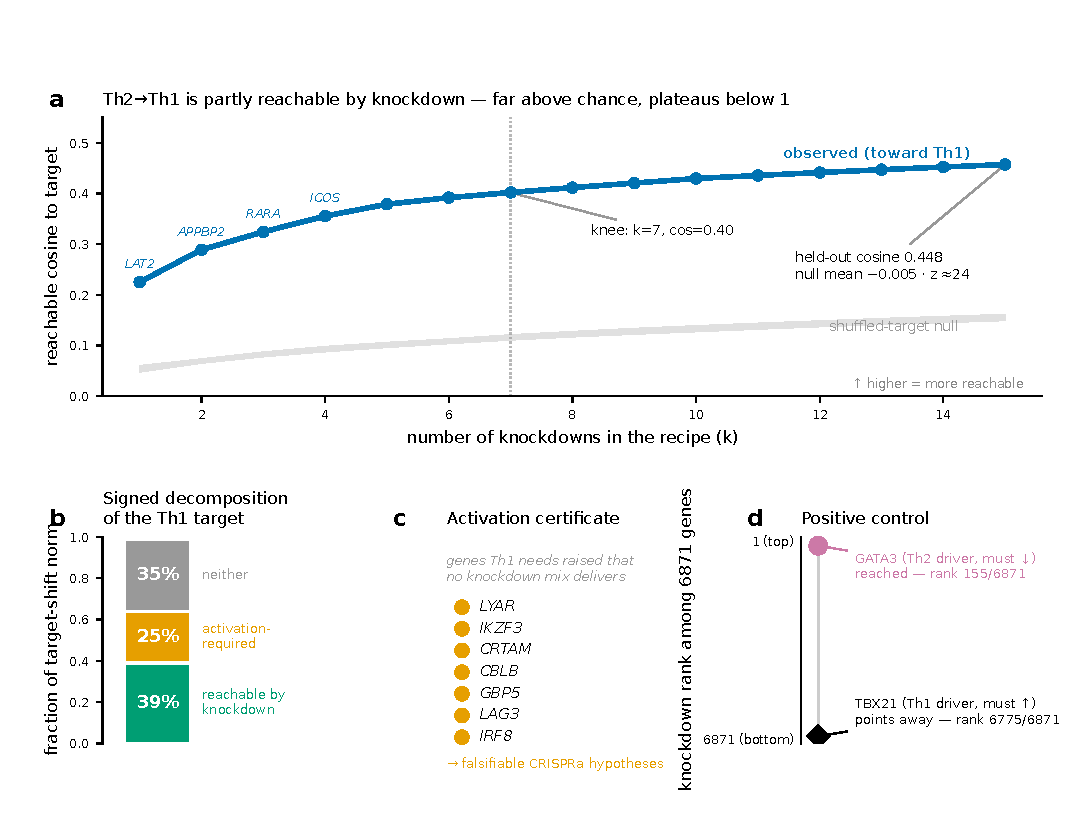
\includegraphics[width=\textwidth]{fig2}
\caption{\textbf{T\textsubscript{H}2$\rightarrow$T\textsubscript{H}1 is partly reachable by
knockdown.}
\textbf{(a)}~Greedy reachability spectrum: reachable cosine versus recipe size $k$, far above
the shuffled-target null at every $k$, with a knee at $k=7$ (cosine $0.40$) and a held-out
cosine of $0.448$ (null mean $-0.005$, $z\approx24$). \textbf{(b)}~Signed decomposition of the
target: $39\%$ reachable by knockdown, $25\%$ activation-required, $35\%$ neither.
\textbf{(c)}~Activation certificate: seven genes the T\textsubscript{H}1 target needs raised
that no knockdown mix supplies---falsifiable CRISPRa hypotheses. \textbf{(d)}~Positive
control: the T\textsubscript{H}2 driver GATA3 is reached (rank $155/6871$) while the
T\textsubscript{H}1 driver TBX21 is correctly anti-aligned (rank $6775/6871$).}
\label{fig:headline}
\end{figure}

\subsection{Knockdown is never the majority modality across a 12-cell atlas}
\label{sec:results-atlas}
To test whether the partial-reachability finding is idiosyncratic to one transition, we ran
the oracle across an atlas of $12$ target cell-states: four transitions
(toward T\textsubscript{H}1, toward T\textsubscript{H}2, toward younger, toward older) under
three activation conditions (resting, stimulated $8$\,h, stimulated $48$\,h). Every one of the
$12$ targets is statistically reachable, with held-out $z$ ranging from $4.7$ to $45.0$; none
is a false positive of the cone's dimensionality. But in no case does loss-of-function account
for the majority of the shift (Fig.~\ref{fig:atlas}a): the mean loss-of-function fraction is
$0.34$, and the knockdown bar never crosses the $50\%$ line. Resting cells are the most
reachable along all four axes---consistent with activation adding gain-of-function directions
that knockdown cannot span---and the verdicts range from ``partially reachable'' (four resting
transitions) to ``weakly reachable'' (the stimulated conditions). The general conclusion is
robust: across transitions, cell states, and activation conditions, engineering by knockdown
alone reaches a real but minority fraction of the desired change, and an honest method must
report that fraction rather than a single reachable/not-reachable bit.

The atlas also exposes a calibration hazard that we report against ourselves
(Fig.~\ref{fig:atlas}b). The in-sample reachable cosine (mean $0.580$) systematically
overstates the held-out-gene cosine (mean $0.355$), by a mean gap of $0.225$ (range
$0.18$--$0.27$) across all $12$ transitions; an $85\%$ without-replacement gene-panel
bootstrap gives tight confidence intervals (e.g. toward T\textsubscript{H}1 resting: point
$0.627$, bootstrap mean $0.639$, CI $[0.633, 0.649]$), confirming that the gap is a real
optimism bias and not estimation noise. We therefore assign a confidence tier to each
transition from its held-out $z$ ($2$ high, $6$ medium, $4$ low) and quote held-out numbers
everywhere. Finally, the closed-form anisotropy null lands almost exactly on the empirical
shuffle null (Fig.~\ref{fig:atlas}c; Pearson $r=0.995$ in-sample, $0.998$ held-out), which is
what makes the atlas-wide analysis affordable.

\begin{figure}[htbp]
\centering
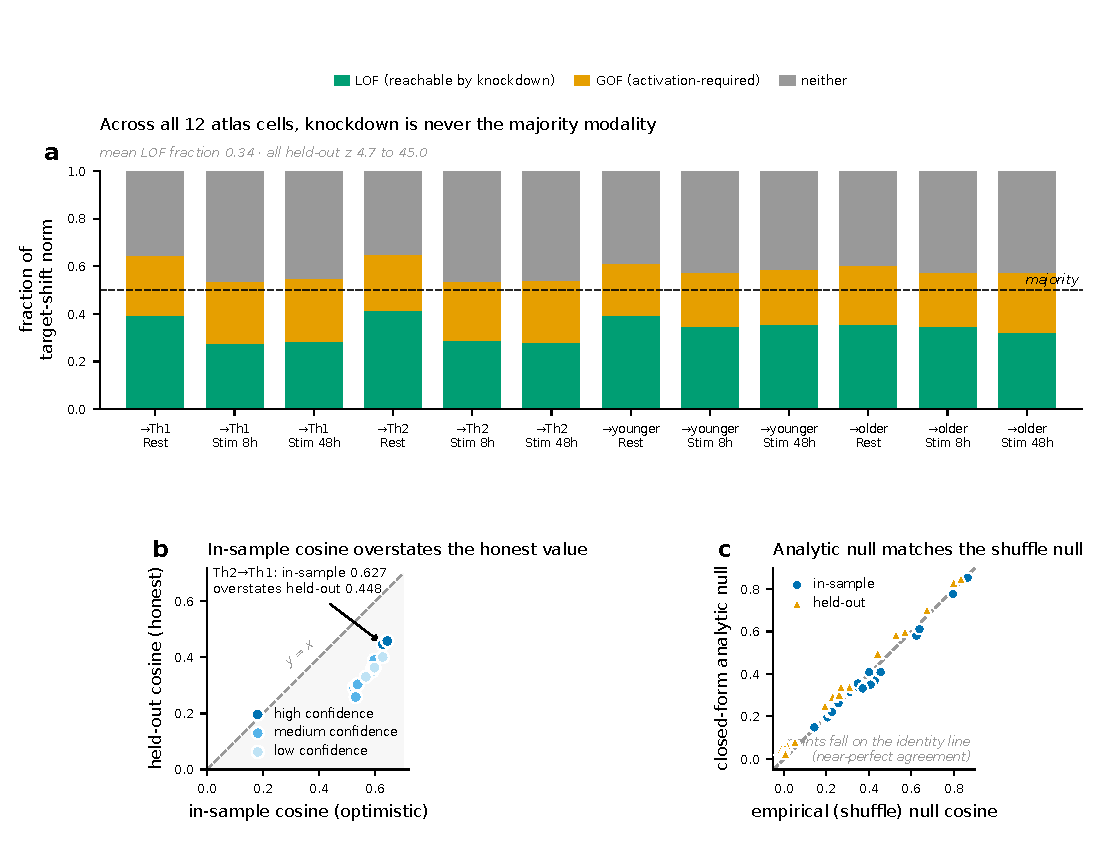
\includegraphics[width=\textwidth]{fig3}
\caption{\textbf{Across a 12-cell atlas, knockdown is never the majority modality.}
\textbf{(a)}~Signed LOF/GOF/neither decomposition for all $12$ targets (four transitions
$\times$ three activation states); the loss-of-function (green) bar never crosses the $50\%$
majority line, mean LOF fraction $0.34$, all held-out $z$ between $4.7$ and $45.0$.
\textbf{(b)}~In-sample reachable cosine overstates the honest held-out cosine on every
transition (points below $y=x$), mean gap $0.225$; marker shade encodes the confidence tier.
\textbf{(c)}~The closed-form analytic null matches the empirical shuffle null
(near-identity), justifying its use atlas-wide.}
\label{fig:atlas}
\end{figure}

\subsection{The verdict survives five reinforcement stress tests}
\label{sec:results-robustness}
A feasibility verdict is only trustworthy if it is not an artifact of a modelling or scoring
choice. Five analyses each attack a different assumption; the headline conclusion---partly
reachable by knockdown, with a named activation remainder---holds under all five, and two of
them \emph{tighten} the original claims rather than merely surviving. The analyses that carry a
dedicated panel appear in Supplementary Figs.~\ref{fig:supp-deg}, \ref{fig:supp-calib},
\ref{fig:supp-split} and~\ref{fig:supp-crossref}.

First, the non-negativity constraint earns its place. Relative to an unconstrained
least-squares fit that is free to run knockdowns in reverse, the biological constraint costs
only a mean of $0.018$ in held-out cosine, yet the unconstrained fit buys that improvement with
$\approx\!3{,}537$ biologically unrealizable negative weights; the cone recovers a mean $95\%$
(range $86$--$103\%$) of the unconstrained cosine and beats the single best generator in all
$12$ cells. The constraint is nearly free and is the sole source of the Farkas/KKT certificate.

Second, the modest absolute cosine is close to its modality-imposed ceiling. Because a
knockdown-only cone cannot express gain-of-function directions, the attainable held-out cosine
is bounded by $\sqrt{\smash[b]{f_{\mathrm{LOF}}}}$; the headline $0.448$ is $71\%$ of that
ceiling (atlas mean $61\%$, range $49$--$71\%$), and the residual gap is $22$--$26\%$
gain-of-function-locked. The ``modest'' number is therefore most of what knockdown can achieve
in principle, not a tuning shortfall.

Third, the recipes are additive-safe with margin. Every recommended knee recipe is additive-safe
in all $12$ cells (per-recipe reliability $0.92$--$0.96$), and the combined-magnitude
saturation cap binds only at $k\approx28$ knockdowns versus a knee of $k\approx4$--$5$---a
$5.6\times$ margin on the headline recipe.

Fourth, and most stringently, the verdict strengthens rather than collapses when the
signal-dilution critique of \citet{Mejia2026} is applied (Fig.~\ref{fig:supp-deg}). Reweighting
the metric by each gene's target magnitude ($w_g=\lvert d_g\rvert$) raises the Tier-2
T\textsubscript{H}2$\rightarrow$T\textsubscript{H}1 reachable cosine from $0.627$ to $0.803$ at
rest (and every stimulated condition and every held-out Norman double likewise increases), while
the held-out $z$ stays far above the significance floor ($28.3\rightarrow14.1$ at rest). The
dynamic-range fraction barely moves ($0.447\rightarrow0.499$) because the shuffled floor rises
in step ($0.346\rightarrow0.619$); the verdict's placement between floor and ceiling is stable,
so it is not a dilution artifact (Fig.~\ref{fig:supp-calib}). The unweighted metric remains the
default and reproduces the published numbers exactly.

Fifth, the certificate is reproducible but its interpretation must be stated carefully
(Figs.~\ref{fig:supp-split}--\ref{fig:supp-crossref}). Under a random gene-axis split the top
certificate genes hold their rank (cross-half Spearman $\rho=0.65$, half-versus-full $0.84$,
$z\approx35$ against a shuffle null of $\approx0$; the full top-$30$ is retained), while the
tail drifts. A retrospective cross-reference of the top $20$ genes, however, qualifies the
biological reading: the highest-demand genes are state-markers (LYAR, CRTAM, GBP5) and
\emph{negative} regulators (IKZF3/Aiolos, CBLB, LAG3)---genes whose \emph{deletion}, not
activation, boosts T-cell function---while the canonical T\textsubscript{H}1 master
transcription factors are present in the certificate but rank deep (IFNG $\#35$, TBX21 $\#144$,
STAT4 $\#364$, STAT1 $\#473$). Of the $20$, four are literature-SUPPORTED, seven PLAUSIBLE, and
nine UNKNOWN, and $8/20$ carry a strong ($\ge0.5$) Open Targets genetic link to a
T\textsubscript{H}1-driven autoimmune disease. We therefore read the certificate as a
reproducible ranking of \emph{unmet upward demand}, not as a validated list of activation
targets: for the negative regulators in particular, the direction of a useful intervention may
be opposite to naive activation. This is a tightening of the original ``activation certificate''
framing, and we carry it into the discussion.

Finally, applying the operator to an independent pair of cell types bounds what transfers, which
we develop next.

\subsection{The operator transfers unchanged to a K562 CRISPRa screen}
\label{sec:results-transfer}
A feasibility operator is only useful if it is not bespoke to one screen. We applied the
identical pipeline---same code, no retuned parameters---to the K562 combinatorial CRISPR
activation screen of \citet{Norman2019} (GSE133344), a different cell type, a different
perturbation direction (activation rather than interference), and a different experimental
design. Holding out the CEBPA master-regulator state as the target, the oracle reaches a
cosine of $0.878$ (residual norm $0.479$) against a shuffled-target null with median $0.389$
and $95$th percentile $0.411$ ($z\approx37$ over $500$ iterations), and a held-out-gene cosine
of $0.856$ ($z\approx23.5$) (Fig.~\ref{fig:transfer}a). The recipe is led by CEBPE, the CEBPA
paralog, with a knee at $k=2$ (CEBPE\,$+$\,SPI1)---a biologically sensible minimal program.
Where the target is not fully reached, the certificate again names an interpretable
program: the CEBPA state requires raising a myeloid-differentiation module (MNDA, HP, VSIG4,
NCF1) orthogonal to what the activation atoms in the screen supply.

Crucially, the Norman screen contains \emph{measured} double perturbations, which let us test
the additivity assumption that underlies every multi-gene recipe rather than merely assert it
(Fig.~\ref{fig:transfer}b). Across $126$ measured doubles, the cosine between the true double
perturbation and the sum of its two singles has median $0.71$: additivity is a good but
\emph{bounded} approximation, not an identity. We characterized the departure directly.
The deficit grows with the combined perturbation magnitude (Spearman $+0.58$), consistent with
a scale-free saturation ceiling ($M^{\star}=13.9$ in units of the median single-effect norm,
fit $R^2=0.57$); the intuitive hypothesis that collinear pairs should be most sub-additive was
\emph{refuted} (Spearman $-0.16$, not significant). The practical consequence, which we carry
into every recipe claim, is that multi-gene knockdown recipes are an extrapolation to be
tested, not an exact prediction, and their reliability degrades at large combined magnitude.

\begin{figure}[htbp]
\centering
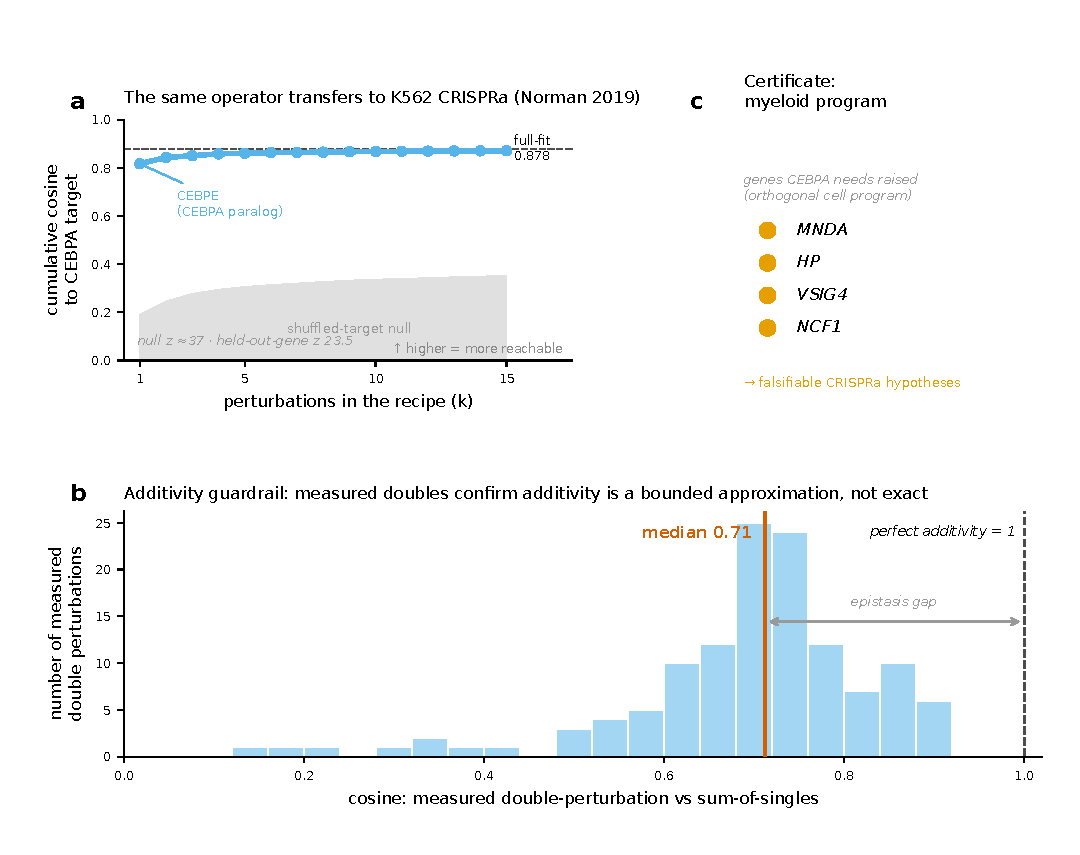
\includegraphics[width=\textwidth]{fig4}
\caption{\textbf{Transfer to Norman 2019 K562 CRISPRa and the additivity guardrail.}
\textbf{(a)}~The unchanged operator reaches the held-out CEBPA state at cosine $0.878$
(full-fit), far above the shuffled-target null ($z\approx37$; held-out-gene $z\approx23.5$),
with the recipe led by the CEBPA paralog CEBPE. \textbf{(c)}~The infeasible remainder's
certificate names a myeloid program (MNDA, HP, VSIG4, NCF1). \textbf{(b)}~Across $126$ measured
double perturbations, the cosine of the measured double to the sum of its singles has median
$0.71$: additivity is a bounded approximation, and the ``epistasis gap'' to perfect additivity
($=1$) is real.}
\label{fig:transfer}
\end{figure}

To probe generalization more systematically than a single held-out state, we applied the
operator to an independent pair of cell types---the genome-scale essential-gene Perturb-seq
screens of \citet{Replogle2022} in K562 and RPE1 cells ($843$ shared single-gene perturbations
over $2{,}832$ shared genes)---and asked, at three levels, what transfers across cell type
(Supplementary Fig.~\ref{fig:supp-transfer}). A single perturbation's effect \emph{direction}
transfers moderately: the matched cross-type cosine has median $0.35$ against a shuffled-gene
null of $\approx0$, rising to $0.64$ along the common essential-stress axis. The reachability
\emph{verdict} transfers only as a graded quantity, not a binary flip---the residual norm is
systematically worse under a cross-type basis than a within-type one ($0.61\rightarrow0.87$ for
K562 targets, $0.37\rightarrow0.68$ for RPE1)---so a naive $100\%$ verdict-agreement rate is an
artifact of an over-expressive $843$-atom cone and should be read as a residual, not a label.
The minimal \emph{recipe} does \emph{not} transfer: the same-target Jaccard overlap across cell
types is only $0.11$, collapsing to the random-selection null ($0.05$) under a cross-type basis.
The prescription is therefore bounded: the \emph{direction} of a cell-state shift is portable
across cell types, but the \emph{specific minimal recipe} is cell-type-specific and must be
re-derived per system. This is a cross-cell-type generalization probe on essential-gene screens,
not a second CD4\textsuperscript{+} T-cell polarization screen.

\subsection{No prior method occupies the measured-effects, verdict-plus-certificate corner}
\label{sec:results-landscape}
We placed the oracle against a structured survey of $92$ methods spanning $2011$--$2026$
(Section~\ref{sec:related}), scored on two axes: how strongly each is grounded in measured
effect vectors, and whether it emits a feasibility verdict with a certificate
(Fig.~\ref{fig:landscape}a). The two capabilities are held by \emph{disjoint} sets of prior
methods. The $14$ methods that operate directly on measured effects are all forward-only
predictors or rankers; none returns a feasibility verdict or a data-grounded certificate. The
$13$--$15$ methods carrying any verdict- or certificate-like output are all model-theoretic---%
their guarantee is a property of a hand-built, fitted, or inferred model, and they span
several families (structural and Boolean network control, control-from-data, an inferred
single-cell GRN, a causally inspired predictor) rather than one. The intersection of
``grounded in measured effects'' and ``emits a verdict plus certificate'' is empty for all
$91$ prior methods; the reachability oracle is the sole occupant of that corner. The
family-level capability matrix (Supplementary Fig.~\ref{fig:supp-matrix}) shows the same
structure per capability column: measured-effect grounding and feasibility output never
co-occur in any prior family.

We state the scope of this claim precisely. It is a claim about the \emph{combination} of two
capabilities on a structured survey, not a claim that any individual capability is
unprecedented; network control has reasoned about reachability for over a decade, and many
methods use measured data. The novelty is the pairing---a feasibility decision computed
directly from measured effects, with a certificate---and the disjointness is the evidence for
it.

\begin{figure}[htbp]
\centering
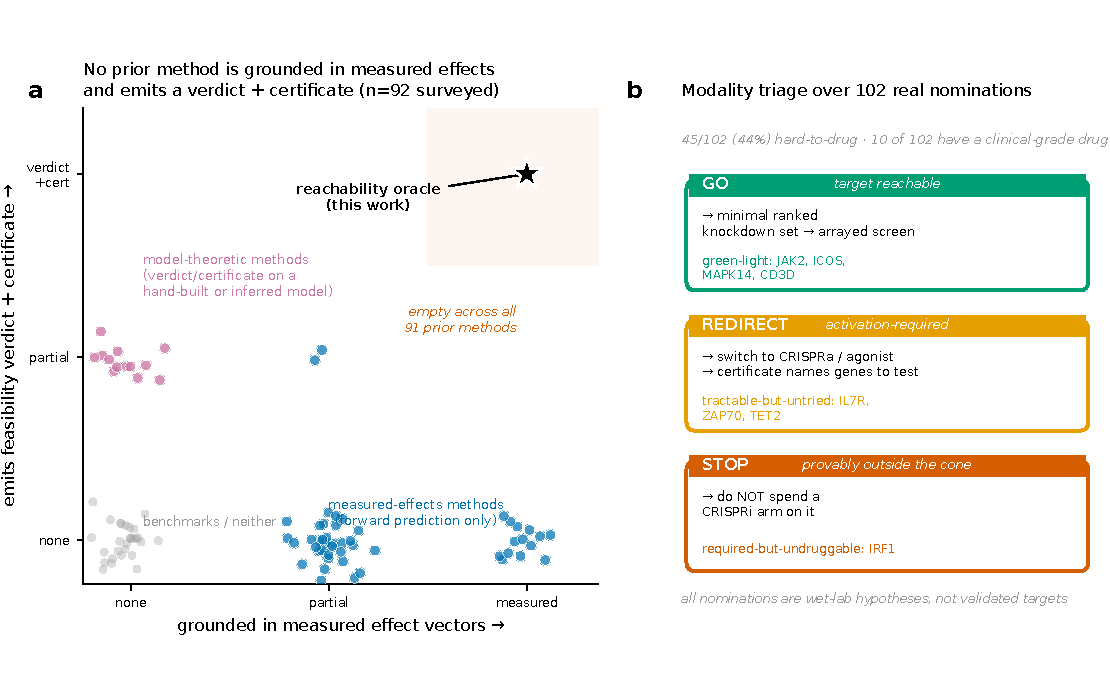
\includegraphics[width=\textwidth]{fig5}
\caption{\textbf{Landscape positioning and modality triage.}
\textbf{(a)}~Each of $92$ surveyed methods ($2011$--$2026$) placed by measured-effect
grounding ($x$) and feasibility-verdict-plus-certificate output ($y$). Measured-grounded
methods (blue) are forward-only; verdict/certificate methods (pink) are model-theoretic; the
top-right corner is empty across all $91$ prior methods and occupied only by this work.
\textbf{(b)}~The verdict translates into a GO/REDIRECT/STOP triage over $102$ real target
nominations ($45/102 = 44\%$ hard-to-drug, $10$ with a clinical-grade drug); all nominations
are falsifiable wet-lab hypotheses, not validated targets.}
\label{fig:landscape}
\end{figure}

\subsection{From verdict to experiment: a GO/REDIRECT/STOP triage}
\label{sec:results-impact}
The point of a feasibility verdict is that it changes what experiment gets run. We applied the
oracle to $102$ real target nominations drawn from the T-cell transitions and translated each
verdict into one of three actions (Fig.~\ref{fig:landscape}b): \textbf{GO}---the target is
reachable, so hand the minimal ranked knockdown set to an arrayed CRISPRi screen;
\textbf{REDIRECT}---the target is activation-required, so switch to a CRISPRa/agonist arm, with
the certificate naming the genes to test first; and \textbf{STOP}---the target is provably
outside the cone, so do not spend a knockdown arm on it. This matters because $45/102$ ($44\%$)
of the nominated targets are hard-to-drug and only $10$ carry a clinical-grade drug, so
misallocating screen arms is expensive. Across transitions, $36$--$49\%$ (mean $\approx42\%$)
of each transition's addressable shift needs induction and is therefore unreachable by a
knockdown-only screen---exactly the fraction a CRISPRi-only campaign would waste effort on
without a feasibility check.

The triage surfaces concrete, and honestly caveated, examples. Nine targets are green-lit as
directly reachable and druggable (including JAK2, ICOS, MAPK14, CD3D). Three are tractable but
untried and flagged for a redirected arm (IL7R, which carries the highest genetic support;
ZAP70; TET2). One, IRF1, is a top T\textsubscript{H}2 knockdown node with strong immune-disease
genetic support but no conventional small-molecule or antibody handle (degrader-only), a
required-but-undruggable case where the verdict argues for a new modality rather than a
conventional campaign. We emphasize that every one of these is a prioritization hypothesis for
the bench, generated by geometry over one screen; none is a validated target, and the oracle's
role is to triage where experimental effort is spent, not to replace the experiment.



\input{sections/40_related_work}

\section{Discussion}
\label{sec:discussion}

We have described a feasibility oracle that treats a genome-scale CRISPRi screen as a
dictionary of measured effect vectors and decides, by convex geometry, whether a target
cell-state shift can be reached by a non-negative combination of knockdowns. The decision is
constructive on both sides: a reachable target returns a minimal ranked recipe, and an
unreachable one returns a Farkas/KKT certificate that names the genes requiring activation.
The value of the framework is not a new list of T-cell regulators---those are already in the
source screens and we use them only as positive controls---but a new \emph{kind of output}:
a falsifiable feasibility verdict computed directly from measured effects, which no method in
a 92-entry survey provides.

\subsection{Interpretation}
Three findings are worth restating for their scientific rather than methodological content.
First, a real polarization shift (T\textsubscript{H}2$\rightarrow$T\textsubscript{H}1) is only
\emph{partly} reachable by knockdown (held-out cosine $0.448$; $39\%$ of the shift in the
loss-of-function cone), and this pattern holds across a $12$-cell atlas where knockdown is
never the majority modality (mean loss-of-function fraction $0.34$). The implication for
practice is direct: a knockdown-only campaign, however well designed, addresses a minority of
most cell-state transitions, and the remaining majority is a mix of required activation and an
irreducible remainder. This gap is not a tuning shortfall: the headline held-out cosine is
$71\%$ of the modality-imposed ceiling that a knockdown-only cone can attain in principle
(atlas mean $61\%$), so most of what loss-of-function can supply is already captured. Second,
the certificate turns this limitation into a plan---it names, reproducibly, which genes carry
the unmet upward demand---so an infeasibility result redirects rather than terminates an
experiment. We are deliberately careful about how that list is read: the highest-demand genes
are state-markers and \emph{negative} regulators rather than the canonical master
transcription factors (which are present but rank deep), so the certificate is a reproducible
statement of \emph{where activation is required}, not a validated list of activation targets,
and for some entries the useful intervention may be opposite in sign to naive activation.
Third, the operator transfers unchanged to screens in other cell types, but transfer is
graded: the \emph{direction} of a cell-state shift is portable across cell types while the
\emph{specific minimal recipe} is not, so the framework is a property of the geometry whose
quantitative recipe must still be re-derived per system.

\subsection{Limitations}
\label{sec:limitations}
The rigor of a feasibility claim rests on being explicit about what it does not establish. We
group the principal limitations by severity; a detailed, actionable reinforcement plan
accompanies this manuscript as a standalone document.

\paragraph{The additivity assumption is load-bearing and only bounded.}
Every multi-gene recipe assumes that co-perturbation effects add. On the $126$ measured
double perturbations available (Norman K562), the measured double aligns with the sum of its
singles at median cosine $0.71$---good, but not exact, and degrading with combined
perturbation magnitude (Spearman $+0.58$ deficit-versus-magnitude; a scale-free saturation
ceiling $M^{\star}=13.9$). The intuitive hypothesis that collinear perturbations should be most
sub-additive was refuted (Spearman $-0.16$, not significant), so the departure is a magnitude
effect, not a redundancy effect. This is the single most important caveat: recipes of more
than a few knockdowns, or knockdowns of individually large effect, are extrapolations whose
error is bounded but real, and the CD4\textsuperscript{+} T-cell dictionary itself contains no
measured doubles with which to check additivity in-domain.

\paragraph{The verdict is robust to measurement error but sensitive to coordinated bias.}
Because the effect vectors are estimates, we ask how far they would have to be wrong to overturn
a verdict, calibrated in units of the measured standard error (an E-value-style sensitivity
analysis). Two failure modes separate cleanly. Resampling every effect within its measured
standard error and re-solving leaves the polarization verdicts intact---the bootstrap
$95\%$ interval of the reachable cosine clears the structure-matched null for both
T\textsubscript{H}1 and T\textsubscript{H}2 (Stim48hr)---so \emph{random} measurement error is
not the threat; undirected noise, if anything, inflates reachability by adding anisotropy that
the null already corrects for. The verdict's genuine exposure is a \emph{coordinated}
systematic bias against the target direction: a worst-case attenuation of only $\approx 8\%$ of
the target-aligned signal ($\approx 0.03$ standard-error units) suffices to flip the
T\textsubscript{H}1 verdict. This is precisely the failure mode a randomized interventional
design is built to exclude, and it is why the design-based identification is load-bearing rather
than incidental. The same analysis flags the imported CD4 aging axes as fragile at the
differentiated state---at Stim48hr they sit below the anisotropy null and should not be read as
reachable---a caveat the raw cosine alone would have hidden.

\paragraph{Loss-of-function has a structural ceiling.}
The modest absolute reachable cosine is not a tuning failure but a property of the modality:
a non-negative combination of knockdowns cannot express directions that require increased
expression, so any target with a substantial gain-of-function component is unreachable by
construction. The knockdown-only ceiling equals $\sqrt{\smash[b]{f_{\mathrm{LOF}}}}$ and
matches the in-sample cone cosine to $10^{-4}$; against it, the headline $0.448$ is $71\%$ of
what is attainable in principle (atlas mean $61\%$, range $49$--$71\%$), with the residual
$22$--$26\%$ gain-of-function-locked. This is why we report a signed decomposition rather than a
single reachability score, and why the honest headline number is well below one \emph{yet}
close to its own ceiling---a distinction we make explicitly so the number is not read as a
failure of fit.

\paragraph{One perturbation system, few donors, collapsed across donors.}
The primary results derive from a single primary-cell system (CD4\textsuperscript{+} T cells)
with four donors, and the effect vectors available to us are collapsed across donors, so we
cannot perform a true leave-one-donor-out generalization test on the primary dictionary.
External validity across genotypes, tissues, and laboratories is therefore asserted by the
cross-dataset transfer to K562, not yet established within the primary system. The
transcription-factor-versus-marker split in the positive-control analysis is likewise a
post-hoc, exploratory annotation rather than a pre-registered test.

\paragraph{Statistical nulls answer narrow questions.}
The shuffled-target null establishes that a target is more reachable than a structure-matched
random direction; it does not establish that the recipe is biologically correct. The
held-out-gene analysis establishes generalization across expression coordinates; it does not
establish generalization across cells or conditions. And the in-sample cosine systematically
overstates the held-out value (mean gap $0.225$ across the atlas), which is why every headline
number in this paper is the held-out one. A separate random-perturbation diagnostic is
negative by construction and is used only as an internal control, not as evidence of
performance.

\paragraph{The certificate is reproducible but not yet a validated target list.}
Under a random gene-axis split the top certificate genes hold their rank (cross-half Spearman
$\rho\approx0.65$, half-versus-full $\approx0.84$, $z\approx35$ against a shuffle null), so the
ranking is a stable property of the data and not of a particular fit. Its \emph{biological}
interpretation is more guarded. A retrospective cross-reference of the top $20$ genes finds
them dominated by state-markers and negative regulators, with the canonical
T\textsubscript{H}1 master transcription factors present but ranked deep; four are
literature-supported, seven plausible, nine unknown, and $8/20$ carry a strong genetic link to
a T\textsubscript{H}1-driven autoimmune disease. We therefore read the certificate as a
reproducible ranking of unmet upward demand, and we flag that for the negative regulators an
``activate this gene'' reading may be directionally wrong---the correct intervention could be
further repression. This cross-reference is exploratory and post-hoc, and it tempers rather
than confirms the earlier ``immunologically credible activation certificate'' framing.

\paragraph{Transfer is graded, and the recipe does not port across cell types.}
Applying the operator to an independent pair of cell types (K562 and RPE1 essential-gene
screens) shows that transfer is a spectrum, not a switch. Single-perturbation effect
\emph{direction} transfers moderately (matched cross-type cosine median $0.35$ versus a
$\approx0$ shuffled-gene null), and the reachability verdict transfers as a graded residual
rather than a binary flip; but the minimal \emph{recipe} does not transfer (same-target
Jaccard $0.11$, collapsing to the random null under a cross-type basis). The apparent
$\approx100\%$ verdict-agreement rate across cell types is an artifact of an over-expressive
$843$-atom cone and must be read as a residual, not a label. The practical bound is that a
recipe derived in one cell type is a hypothesis, not a prescription, in another.

\paragraph{The verdict is robust to the choice of evaluation metric.}
Uniform-gene metrics can in principle dilute a real signal by averaging over unchanged genes.
Reweighting every metric by target magnitude ($w_g=\lvert d_g\rvert$)---the correction called
for by \citet{Mejia2026}---\emph{strengthens} rather than weakens the headline verdict (Tier-2
rest reachable cosine $0.627\rightarrow0.803$; held-out $z$ remains far above the significance
floor), and the calibrated dynamic-range placement is stable because the shuffled floor rises
in step. We report the unweighted metric as the default because it reproduces the published
numbers exactly, but the conclusion does not depend on that choice.

\subsection{Outlook}
The most valuable next experiments follow directly from the limitations. Measuring a modest
panel of double knockdowns in the primary CD4\textsuperscript{+} system would replace the
borrowed K562 additivity estimate with an in-domain one and calibrate the recipe-size ceiling.
Running one CRISPRa arm against a certificate's named genes would provide the first direct test
of an infeasibility prediction---the framework's most distinctive and least-validated claim.
And extending the dictionary to additional cell types and donors would convert the transfer
result from an existence proof into a generalization curve. In each case the framework's
output is what makes the experiment efficient: it says not only what to test but where testing
is unnecessary. We therefore position the oracle as an experiment-triage instrument---a way to
decide where a screen should spend its arms and where it should stop---rather than a
target-validation engine, and we release it in that spirit.

\paragraph{A causal-inference agenda.}
Read as a causal-inference method, the oracle is a design-based counterfactual query: the effect
vectors are average treatment effects from a randomized CRISPRi experiment, and a reachability
verdict asks whether a non-negative compound intervention exists that points at the target state.
That framing makes the identifying assumptions explicit and turns each into a concrete next
experiment. Four are worth naming. First, \emph{interference} (SUTVA): pooled Perturb-seq lets a
perturbed cell's secreted cytokines alter a neighbour's state, which would bias the very
polarization effects the target axis is built from; an arrayed-versus-pooled or MOI-titration
screen would bound this spillover directly and is the primary external-validity test. Second,
\emph{mediation}: decomposing a recipe's effect through master-regulator intermediates would
distinguish a direct lever from one acting only through a downstream factor, sharpening the
minimal recipe into a mechanistic one. Third, \emph{dynamics}: the current verdict is static,
whereas differentiation is a trajectory, so a time-resolved dictionary with g-methods (accounting
for time-varying confounding) would convert a reachability verdict into a reachable
\emph{schedule}. Fourth, \emph{transportability}: the aging axis in particular is a direction
imported from a different population, so a selection-diagram analysis would state which effects
are licensed to transport and re-express the aging verdict as a transported rather than
assumed-invariant quantity. The computable half of this agenda---sensitivity radii, negative-control
outcomes, signed construct validity, weak-instrument-robust recipe intervals, and the
instrumental-variables treatment of guide non-compliance---is already implemented as a
causal-validation dossier accompanying the code; the four experiments above are its wet-lab
continuation.



% ---- Bibliography ----
\FloatBarrier
\bibliography{references}

\clearpage
\appendix
\input{sections/90_supplement}

\end{document}
